\section{Mesures sous Linux}
\subsection{Programme $carrelinux-comedi.c$}
Ce premier programme est un générateur de signal carré. Il va nous permettre d'analyser les réponses temps réel de en étant basé sur Linux. Notre première analyse du programme donne :\begin{itemize}
\item Fonction \emph{Void out} : envoie un signal inverse  celui qu'elle envoyait précédemment. La fréquence semble être défini ailleurs dans le programme. Le signal est envoyé vers le port 0 de la carte E/S initialisé dans la fonction \emph{main}.
\item \emph{Carte E/S} : la librairie $Comedio$ permet d'ouvrir la connexion série avec la carte d'entrée sortie puis d'initialiser le sens du port.
\item \emph{main} : Initialisation d'une structure de temps dans le main qui sera utilisé dans la boucle infinie du programme principal.
\end{itemize}
Le programme entre ensuite dans une boucle infinie dans laquelle il attend un temps \emph{TIMER\_ABSTIME} pour ensuite appeler la fonction \emph{out}. Après, le programme calcule le \emph{next shot}, i.e le prochain déclenchement, qu'il devra attendre lors du recommencement de la boucle.

Avec ce recueil d'informations, nous sommes capable de définir la fréquence du signal du signal carré que nous allons observer : elle est égale à 2 fois le \emph{next shot} calculé dans la boucle infinie : ce calcul est : $next\_shot = 50 000 + t$, la variable $t$ appartient à la structure de temps et elle est défini en nanosecondes donc : \begin{equation}
f = 2\times 50 000ns \Leftrightarrow f= 100\mu s
\end{equation} 

\subsection{Mesures des période du signal}
Pour mesurer les modifications de période, nous avons crée deux variables de type $timespec$ : une qui mesure le temps précédent le sleep, une qui mesure a la fin de l'instance $while(1)$. La mesure de la demi-période du signal carré $\delta$ est alors la différence entre le temps du début de la boucle et le temps en fin de boucle.  

Pour permettre un affichage correct, nous avons introduit dans notre programme une fonction qui permet d'écrire dans un fichier les 5000 dernières $\delta$ mesurées et qui sera appelé dès que le signal \textbf{Ctrl+C} grâce à l'instruction : 
\begin{lstlisting}[style = customc]
signal(SIGINT, IntHandler)
\end{lstlisting} 
Nous utilisons ensuite le fichier de mesure en .res pour un affiche avec un script $gnuplot$. Nous observons les résultats suivants :
\begin{center}
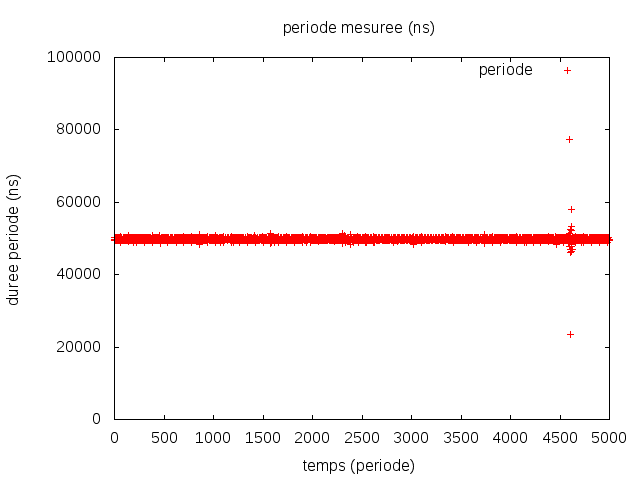
\includegraphics[width = .8\textwidth]{./I/images/delta_no_perturb.png}
\captionof{figure}{Mesure des périodes sans perturbation}
\end{center}

Pour cette première observation, nous n'avons pas touché le système d'exploitation pendant la mesure des périodes et cependant, nous remarquons que celles ci ont eu out de même quelques légères perturbations. Nous allons maintenant effectué quelques perturbations pendant que le relevé s'effectue. 

\begin{center}
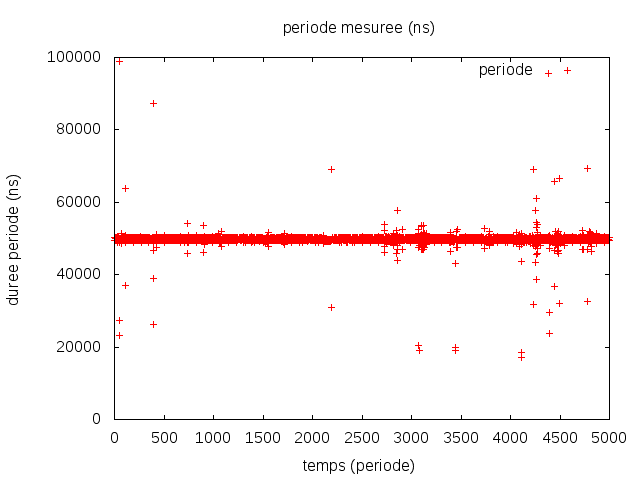
\includegraphics[width = \textwidth]{./I/images/delta1.png}
\captionof{figure}{Mesures des périodes avec quelques perturbations}
\end{center}
Nous notons ici que les petites perturbations commencent à avoir de grosse conséquence sur la demi période du signal. Ces perturbations se notent aussi sur l'oscilloscope où nous observons des modifications du signal. Pour terminer cette étude, nous effectuons une dernière mesure des périodes dans laquelle nous demandons au système d'exploitation une concaténation de fichier volumineux. 


\begin{center}
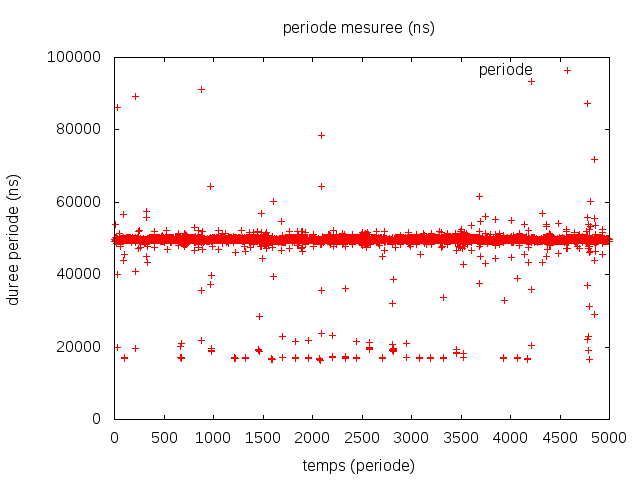
\includegraphics[width = \textwidth]{./I/images/delta_cat.png}
\captionof{figure}{Mesures des périodes avec la commande "cat /dev/zer > file2delete" en parallèle}
\end{center}

Nous observons que la dispersion des périodes est beaucoup plus importante. Le système d'exploitation n'a pas réussi à ordonnancer notre programme avec l'instruction que nous lui avons demandé. De telles différences ne sont pas acceptables pour des applications ou des systèmes Temps Réel. Le système d'exploitation Linux seul ne peut pas être utilisé tel quel pour le Temps réel, nous devons ajouter au noyau la capacité à préempter des tâches avec l'architecture logicielle RTAI.